 \newchapter{feedforward}{Latest Feedforward Results}

This is the introductory text.

\newsection{jitterRecord}{Lowest Achieved Phase Jitter}

The results presented in this section show the best downstream phase jitter currently achieved at CTF3 with the PFF correction. The dataset was taken on Friday 20th November 2015 at 15:38 as one of a sequence of short measurements fine-tuning the gain around the optimal value. Results from the other datasets in this sequence are discussed in the following section to demonstrate the phase stability achieved on longer time scales. The 15:38 dataset shown here comprises 150 pulses taken in interleaved mode, with the correction applied to the 75 odd indexed pulses and no correction applied to the remaining 75 even indexed pulses. The used gain in FONT5a units was 800, corresponding to a real applied correction of 1.13 times the upstream phase using the conversion factor calculated in Section \ref{ss:fontSetup}.

Naturally, this dataset was taken during the best beam conditions currently achieved at CTF3 in terms of phase propagation, taken just after a series of R56 and beam energy optimisations using the same methods discussed in Chapter \ref{c:phasePropagation}. In particular, the first attempt to smooth the upstream phase along the pulse by adjusting the waveform of the first klystron in the CTF3 injector (MKS02) as described in Section \ref{ss:t566Mitigation} yielded the highest upstream-downstream phase correlation achieved to date in normal conditions (higher correlations can be achieved by adding an additional jitter source upstream, as seen in Section \ref{s:pffNovelSetups}). 

Initially considering the mean pulse phase, the correlation with the PFF correction off in this dataset, as shown by the blue distribution of points in Figure \ref{f:BestFF_Real}, is \(0.93\pm0.04\). This gives a theoretical limit of a factor \(2.7\pm0.4\) reduction in the downstream jitter using Equation \ref{e:theoretJitOptGain}. The achieved uncorrected downstream mean phase jitter of \(0.74\pm0.06^\circ\) and downstream-upstream jitter ratio of \(1.1\pm0.1\) are also the lowest achieved at CTF3 to date. With this initial jitter and the theoretical reduction factor of \(2.7\pm0.4\) the lowest corrected downstream jitter that could be achieved is then \(0.27\pm0.05^\circ\). The aforementioned correlation and jitter ratio combine to give an optimal gain of \(1.0\pm0.1\) (Equation \ref{e:theoretOptGain}). With the actual gain used being 1.13 the PFF system would have been slightly over-correcting the downstream phase in these conditions, although the two values are almost consistent within the error bars and the achievable jitter degrades slowly about the optimal value so the effect should be negligible (Section \ref{ss:theoryJitter}) [TODO: Elaborate].

\begin{figure}
  \centering
  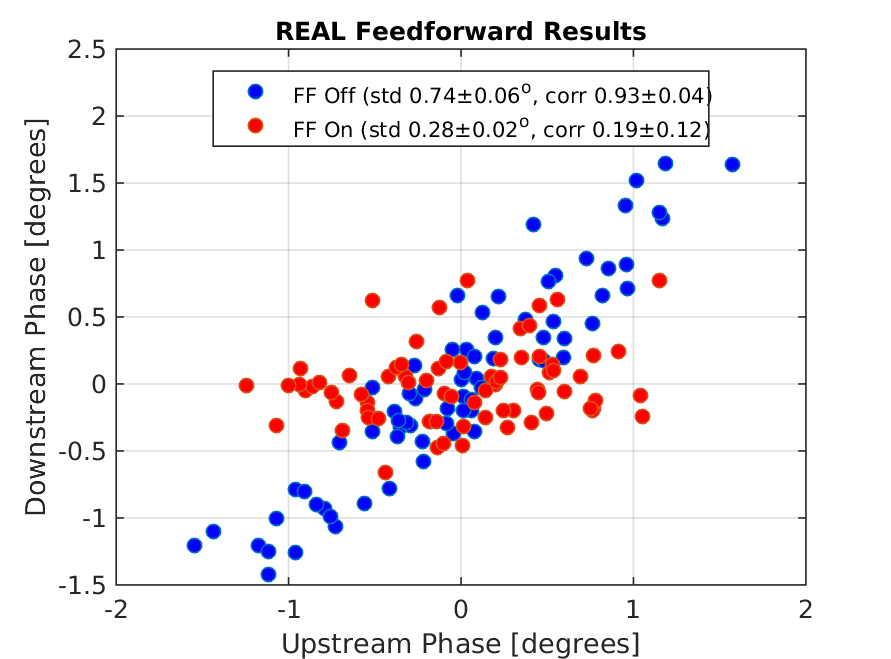
\includegraphics[width=0.75\textwidth]{Figures/feedforward/BestFF_Real}
  \caption{Mean phase.}
  \label{f:BestFF_Real}
\end{figure}

The red distribution of points in Figure \ref{f:BestFF_Real} then shows the effect of the PFF correction on the phase distribution. The correction acts to remove all correlation between the upstream and downstream phase, rotating the distribution as seen in the plot. The correlation is reduced from \(0.93\pm0.04\) to \(0.19\pm0.12\). As the used gain was slightly larger than optimal, a negative correlation might have been expected but this is not the case [TODO: why?]. The downstream phase jitter is reduced from \(0.74\pm0.06^\circ\) to \(0.28\pm0.02^\circ\), a reduction of a factor \(2.6\pm0.3\).  Within the error this agrees perfectly with the theoretical limit derived previously given the beam conditions in this dataset. It should be noted, however, that the measured upstream jitter of \(0.57\pm0.05^\circ\) across the pulses with the PFF correction on in this dataset is lower than the \(0.69\pm0.06^\circ\) measured with the PFF system off (Table \ref{t:BestFF}). This is simply a statistical effect rather than being a systematic difference between the odd and even pulses or an effect of the correction (which can only influence the downstream phase). Assuming the PFF on upstream jitter propagated downstream with the same ratio as the PFF off data, the true `natural' downstream jitter without the correction applied would have been \(0.61\pm0.09^\circ\) and the true factor reduction in the corrected jitter achieved with the PFF system would be decreased to \(2.2\pm0.4\). Assuming the upstream-downstream phase correlation was also not affected by this statistical fluctuation (so that the theoretical jitter reduction of a factor \(2.7\pm0.4\) still holds), a corrected jitter of \(0.23\pm0.05^\circ\) would have been theoretically possible for the PFF on pulses in this dataset. 

[TODO: Distribution of points at around 0.5 degrees downstream?]


With interleaved data it is also possible to simulate the expected effect of the correction empirically, as an additional point of comparison between the achieved and expected results plus as a verification of the theoretical predictions. The distribution of simulated corrected phases is shown in green on Figure \ref{f:BestFF_Simulated}. It is derived by taking the initial distribution with the PFF system off (blue points) and subtracting the upstream phase, multiplied by a gain factor, from the downstream phase. This exactly mimics what the feedforward system would have done if it had been applied to the even pulses in this dataset, and can be directly compared to the odd pulses taken at the same time with the real correction applied. In this example the simulation shown is the ideal case, considering a correction with infinite range and bandwidth applied with the optimal gain. As expected the simulated corrected downstream jitter of \(0.27\pm0.02\) agrees perfectly with the theoretical prediction of \(0.27\pm0.05^\circ\) previously derived. The achieved jitter of \(0.28\pm0.02\) matches both the theoretical and simulated jitter predictions within the error, giving confidence that the overall PFF setup in this dataset (after all the commissioning steps discussed in Chapter \ref{c:commissioning}) was close to optimal. There is perhaps some room for improvement due to the difference between the upstream jitter in the PFF on and off data, as mentioned previously, and this will be elaborated on in Section \ref{s:longPFF} below. Nevertheless, this result clearly demonstrates stability on the mean pulse phase approaching the CLIC target of 0.2 degrees at 12~GHz and demonstrates that achieving this stability with a PFF system is feasible.


\begin{figure}
  \centering
  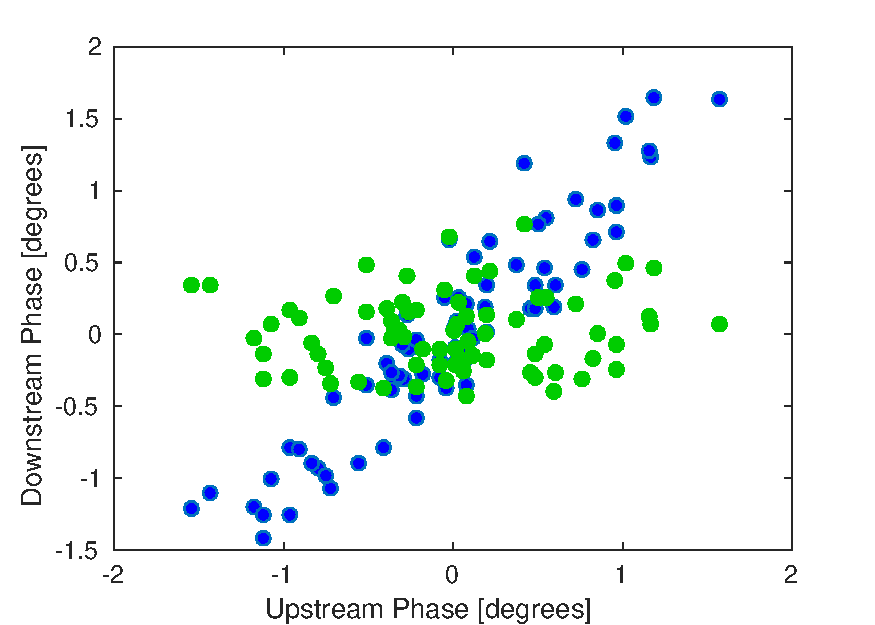
\includegraphics[width=0.75\textwidth]{Figures/feedforward/BestFF_Simulated}
  \caption{Simulated PFF.}
  \label{f:BestFF_Simulated}
\end{figure}


\begin{table}
  \begin{center}
    \begin{tabular}{| c | c | c | c |}
	   \hline
       Correction Status & Upstream Jitter & Downstream Jitter & Correlation \\ \hline
       FF Off & \(0.69\pm0.06^\circ\) & \(0.74\pm0.06^\circ\) & \(0.93\pm0.04\) \\
	   FF On & \(0.57\pm0.05^\circ\) & \(0.28\pm0.02^\circ\) & \(0.19\pm0.12\) \\
	   FF Simulated & \(0.69\pm0.06^\circ\) & \(0.27\pm0.02^\circ\) & \(0.06\pm0.12\) \\ \hline
    \end{tabular}
    \caption{Best PFF results.}
  	\label{t:BestFF}
  \end{center}
\end{table}

Moving on to the stabilisation of the phase along the pulse, Figure \ref{f:BestFF_MeanPhaseAlong} shows the mean phase along the pulse upstream, downstream with the PFF system off and downstream with the PFF system on. The vertical black lines mark the sample range that was used to calculate the mean phase results presented previously. The range is chosen to cover the maximal proportion of the pulse within which the the correction is not being saturated as a result of the phase sag (plus jitter) exceeding the \(\pm6^\circ\) correction range. It covers a total of 81 samples at 5.2 ns per sample, giving a total time span of 422~ns. The demonstration of \(0.28\pm0.01^\circ\) mean phase stability is therefore already on a much longer pulse than is needed for CLIC, where the combined pulse length is only 240~ns. [TODO: Any significant reduction in measured jitter by using 240ns window?] With the optimised phase propagation in place the overall shape of the upstream and (uncorrected) downstream phase, in green and blue respectively, along the pulse are very similar, although small uncorrelated variations are still visible. These uncorrelated differences are then visible in the corrected downstream phase (in red), although the overall ability of the PFF system to flatten the CTF phase sag within the sample range is strikingly clear. The original peak-to-peak variation in the mean downstream phase along the pulse of \(5.76\pm0.14^\circ\) with the correction off is reduced to \(0.65\pm0.07^\circ\) degrees with the correction applied.

\begin{figure}
  \centering
  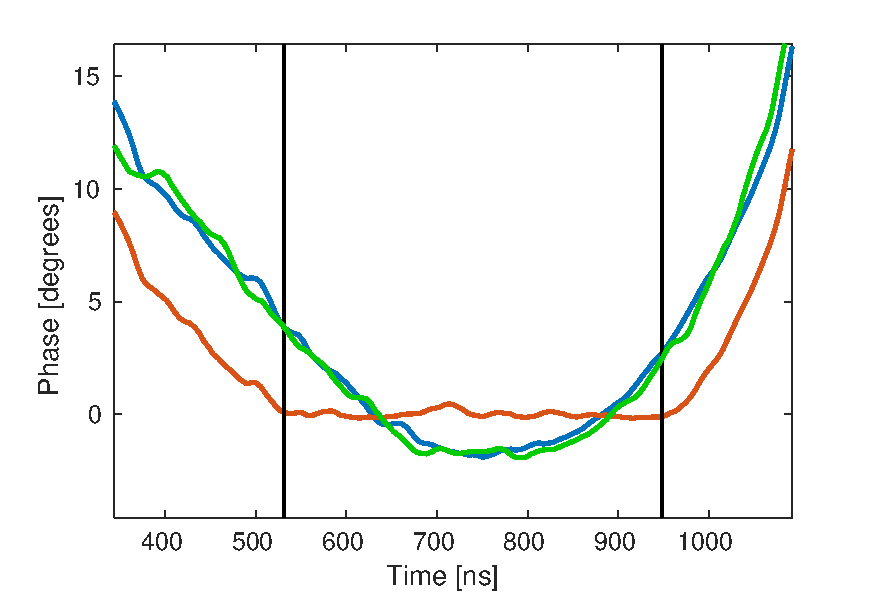
\includegraphics[width=0.75\textwidth]{Figures/feedforward/BestFF_MeanPhaseAlong}
  \caption{Mean phase along.}
  \label{f:BestFF_MeanPhaseAlong}
\end{figure}

Figure \ref{f:BestFF_Flatness} expresses the effect of the PFF system on the phase along the pulse in terms of the distribution of `flatness' values for each pulse in the data set with PFF system off and on. For each pulse, the flatness value is defined as the standard deviation of phase values across the sample range. In this case the flatness value of each pulse therefore corresponds to the standard deviation of 81 values (the length of the sample range). A pulse with a flatness value of zero would have constant phase across the whole sample range, with no small variations such as those seen in Figure \ref{f:BestFF_MeanPhaseAlong}. The value is also insensitive to the jitter on the overall mean pulse phase seen earlier in Figure \ref{f:BestFF_Real}. In Figure \ref{f:BestFF_Flatness}, the uncorrected downstream pulse flatness, dominated by the phase sag at CTF3, of \(1.68\pm0.02^\circ\) is reduced to \(0.26\pm0.01^\circ\) with the correction applied. On average, the corrected pulses are \(6.5\pm0.3\) times `flatter' than the uncorrected pulses.

\begin{figure}
  \centering
  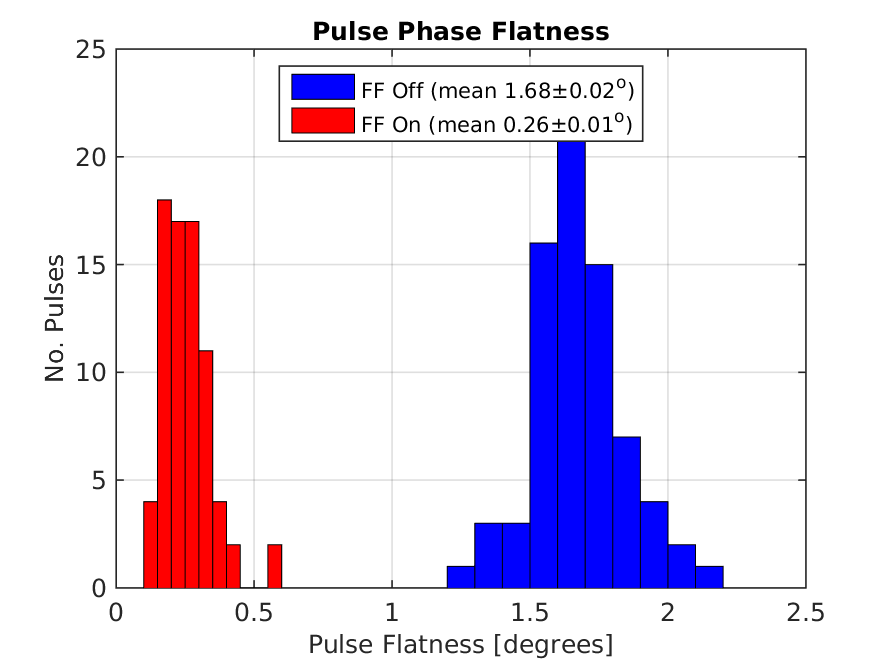
\includegraphics[width=0.75\textwidth]{Figures/feedforward/BestFF_Flatness}
  \caption{Flatness.}
  \label{f:BestFF_Flatness}
\end{figure}

Finally, Figure \ref{f:BestFF_StdPhaseAlong} shows the overall phase jitter at each sample along the pulse upstream and downstream with the PFF system off and on. These jitter values contain components coming from both the jitter on the overall mean pulse phase discussed initially and from the variations along the pulse (the non-zero flatness of each pulse). These jitter values are therefore larger and taking the mean sample jitter within the sample range an initial downstream jitter of \(0.72\pm^\circ\) is reduced to \(0.36\pm^\circ\) by the correction in this case, a factor 2 reduction. There are also variations of up to a factor 2 in the jitter that was achieved at each sample point, the lowest jitter being \(0.27\pm^\circ\) at time 797~ns on the x-axis and the worst \(0.52\pm^\circ\) at time 552~ns. The achieved jitter along the pulse within the sample range also agrees with the simulated result of \(0.38\pm^\circ\) using the interleaved pulses without the correction applied, as shown in Figure \ref{f:BestFF_SimStdPhaseAlong}.[TODO: Error bars] Again, outside the sample range the real system can not match the unlimited range simulation as the phase sag along the pulse saturates the correction. 

[TODO: Why variations in jitter along pulse?]

\begin{figure}
  \centering
  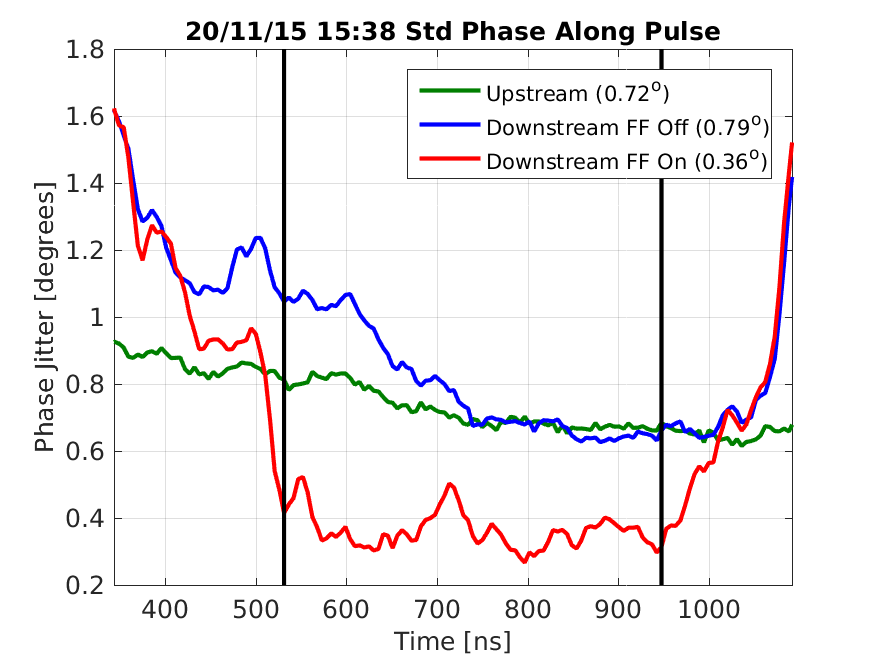
\includegraphics[width=0.75\textwidth]{Figures/feedforward/BestFF_StdPhaseAlong}
  \caption{Std phase along.}
  \label{f:BestFF_StdPhaseAlong}
\end{figure}

\begin{figure}
  \centering
  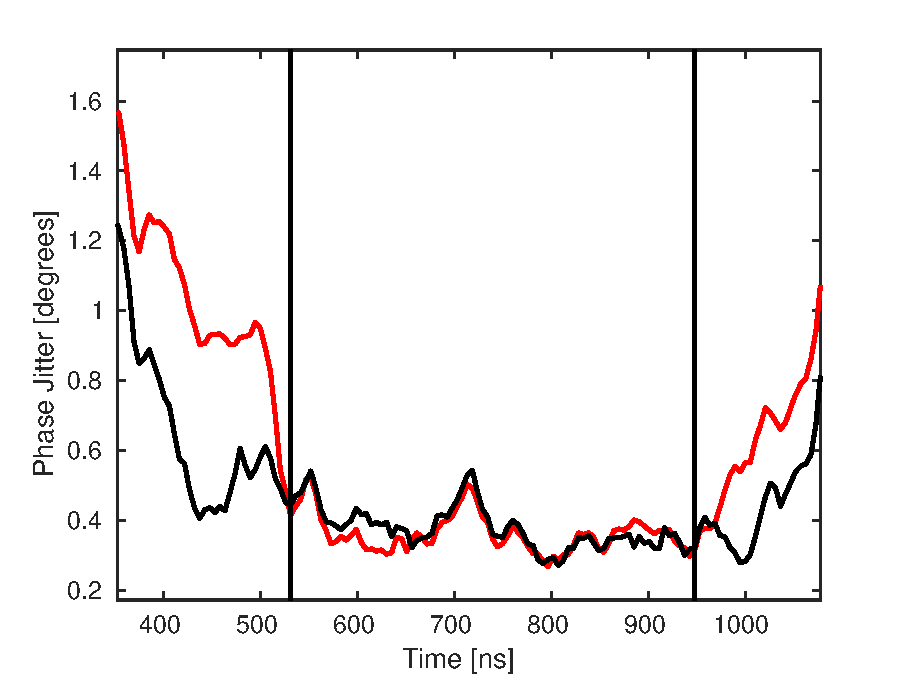
\includegraphics[width=0.75\textwidth]{Figures/feedforward/BestFF_SimStdAlongPulse}
  \caption{Std phase along.}
  \label{f:BestFF_SimStdPhaseAlong}
\end{figure}

\newsection{longPFF}{Correction on Longer Time Scales}

At CLIC 0.2 degrees phase stability would clearly have to be maintained for much longer time scales than a few minutes. This section therefore discusses the status of the correction across longer time scales, demonstrating both the level of corrected phase jitter that can currently be achieved routinely and to highlight areas where improvements are still needed both in the PFF setup itself and the beam conditions. 

The data used is from around 15:25 to 18:05 on the 20th November 2015, the same day as the record result previously shown which was taken during this period at 15:38. The PFF system was not operated continuously throughout this two and a half hour window but 15 individual datasets of a few hundred pulses each were taken and these results have been combined to create a large sample of 3083 interleaved pulses (1541 with the correction on and 1542 with the correction off). The raw history of the mean phases upstream and downstream with the correction on and off in the combined data are shown in Figure \ref{f:longFF_noMeanSubHistory}. The time span of each individual dataset is marked by vertical black lines and the times displayed on the plot represent the start time of each dataset. [TODO: Pulse no. from 1-3083 rather than 1-1500 and offset odd/even by one]. Note that the large jump in the downstream phase between the 16:00 and 16:04 datasets was caused by changes made to magnetic correctors in the TL2 chicane in order to re-optimise the beam orbit and transmission to the downstream phase monitors at this time. In Figure \ref{f:longFF_histDownstreamPhase} the mean phase is subtracted (separately for the upstream, downstream FF off and downstream FF on phase) from each dataset to remove this effect, making a comparison between datasets easier. It is important to emphasise that, apart from this jump in the downstream phase, the overall picture is a fair reflection of the (uncorrected) phase stability at CTF3 in optimal conditions. 

\begin{landscape}

\begin{figure}
  \centering
  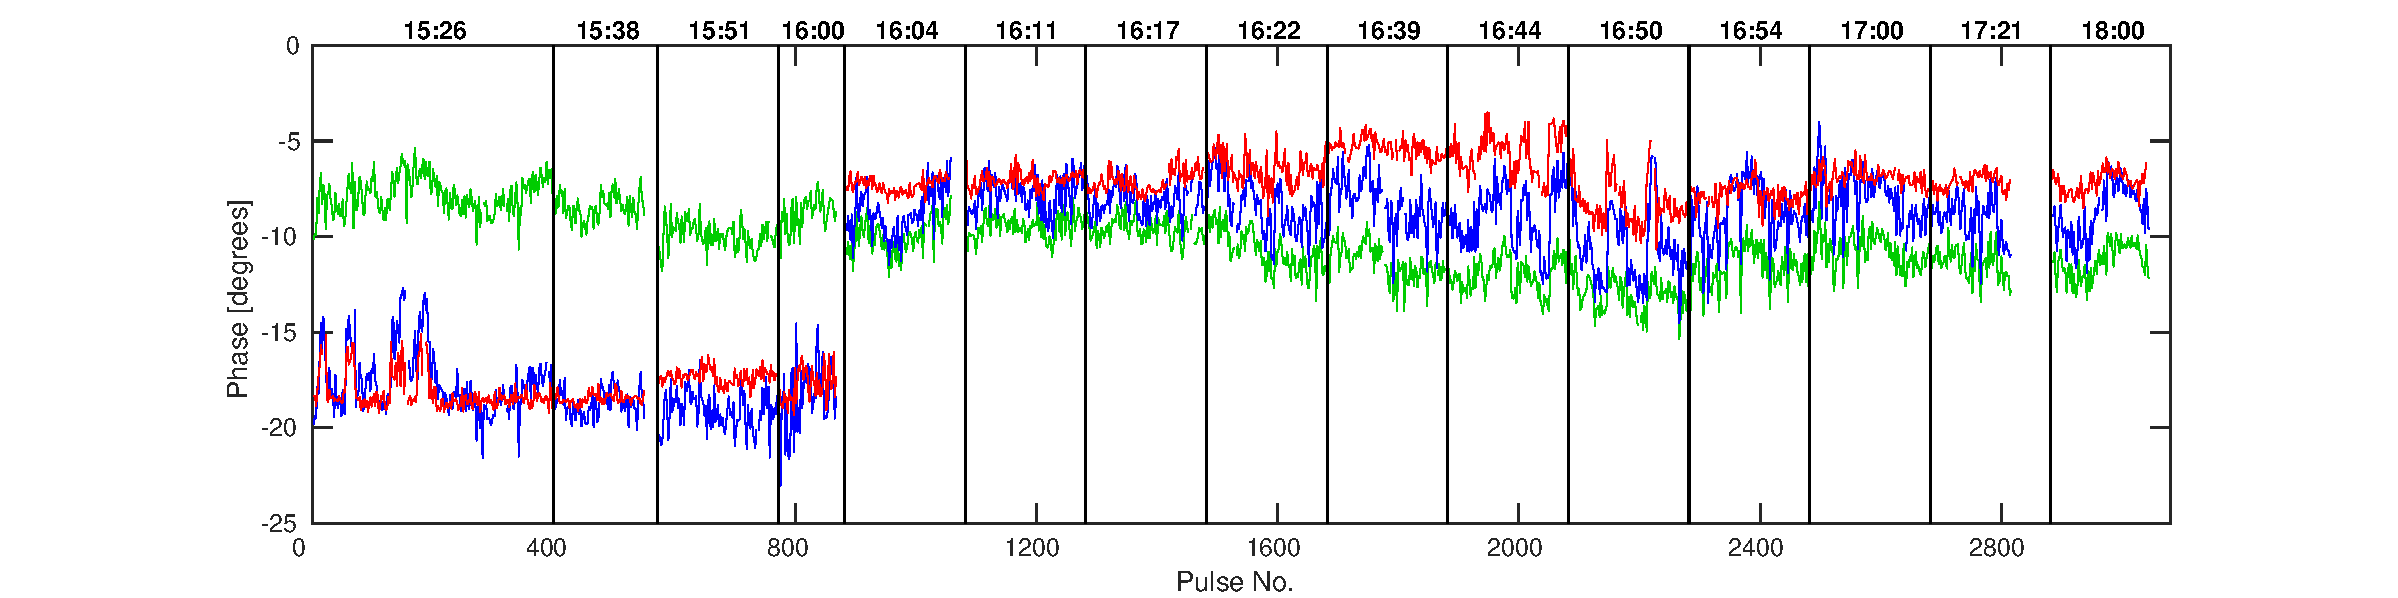
\includegraphics[width=\hsize]{Figures/feedforward/longFF_noMeanSubHistory}
  \caption{History of mean phase across datasets.}
  \label{f:longFF_noMeanSubHistory}
\end{figure}


\begin{figure}
  \centering
  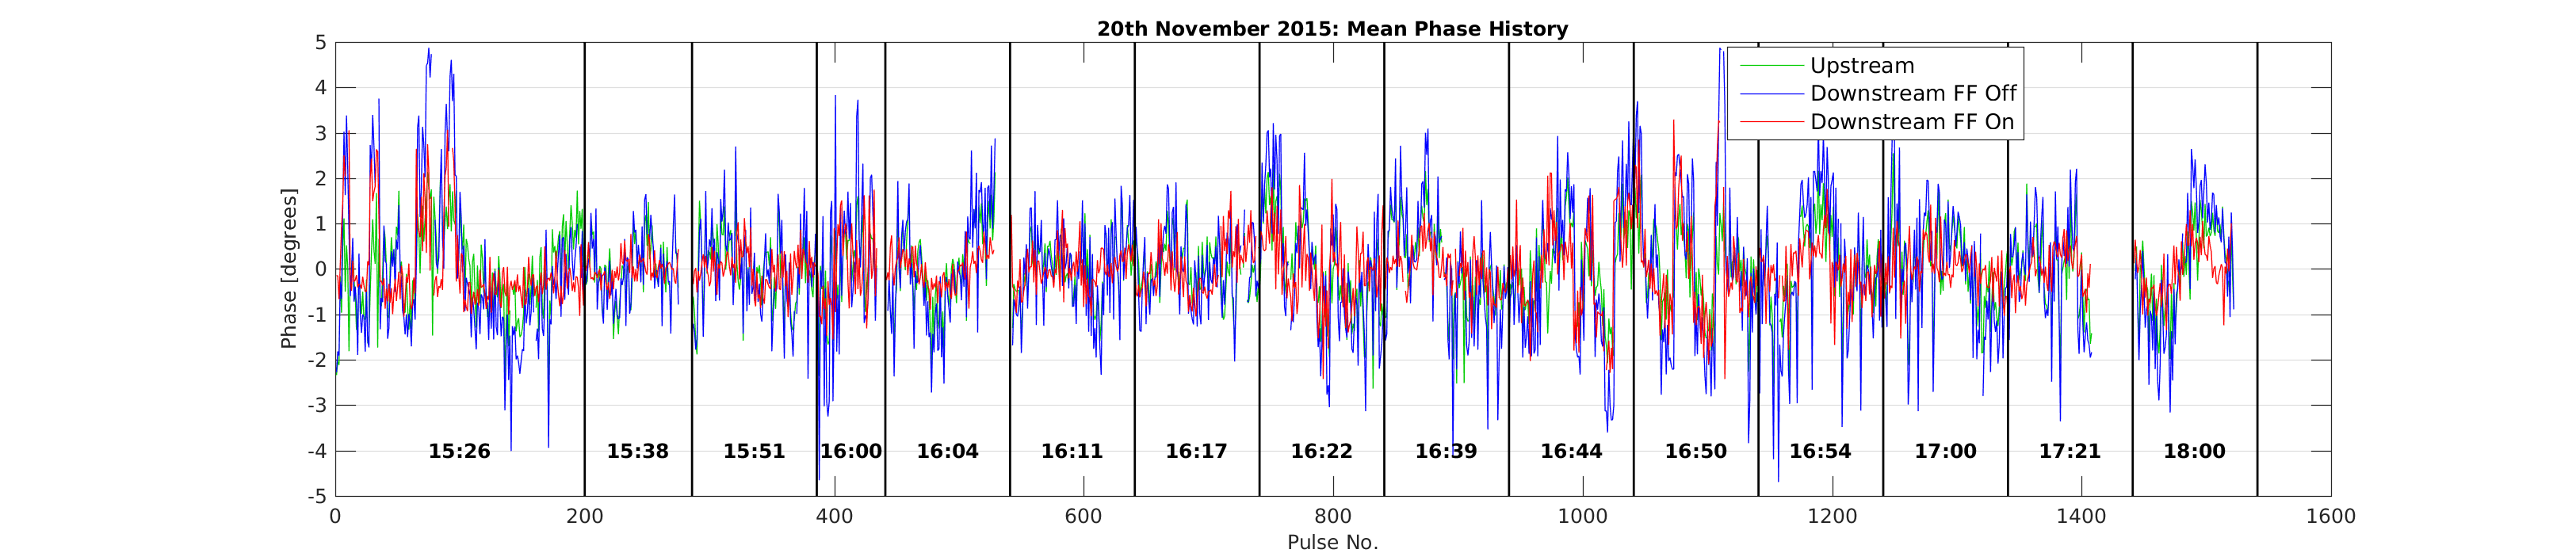
\includegraphics[width=\hsize]{Figures/feedforward/longFF_history}
  \caption{History of mean phase across datasets, with mean subtraction.}
  \label{f:longFF_history}
\end{figure}

\end{landscape}

\subsection{Upstream Phase Drifts}
\label{ss:longFF_upDrifts}

Over the course of the afternoon the mean upstream phase, in green, varies by ten degrees peak-to-peak or \(1.75 \pm 0.02^\circ\) in terms of jitter (Figure \ref{f:longFF_noMeanSubHistory}). [TODO:Source of drift, comment on feedbacks]. Small drifts of up to a few degrees in the upstream phase are not an issue for the performance of the PFF correction providing the correlation between the upstream and downstream phase is not degraded. In some cases upstream phase drifts may lead to a loss in correlation, this could be the case if the source of the drift is a variation in beam energy due to the issues discussed in Chapter \ref{c:phasePropagation}, for example. The variation of the correlation between datasets is discussed later in this chapter.

Larger changes in the upstream phase such as the ten degree fluctuation seen here may also impact the PFF performance purely via the limited correction range of \(\pm6^\circ\) combined with the phase sag along the CTF pulse. Indeed the PFF prototype's main purpose is not to remove any large, slow phase drifts but rather the faster pulse-to-pulse jitter and high frequency variations along the pulse. The phase offset applied by the PFF correction at each sample along the downstream phase, \(\Delta\phi_d(t)\), is given by:

\begin{eqnarray}
	\Delta\phi_d(t) = \begin{cases}
	-6^\circ, &  \text{if $g\phi_u(t) \geq+6^\circ$.}\\
	+6^\circ, &  \text{if $g\phi_u(t)\leq-6^\circ$}.\\
	-g\phi_u(t), &  \text{otherwise.}
	\end{cases}
	\label{e:limCorrection}
\end{eqnarray}

Where \(\phi_u(t)\) is the upstream phase at each sample point and \(g\) is the gain factor used. As the optimal gain (Section\ref{ss:theoryGain}) for the correction is typically larger than one due to the slight amplification in the downstream phase jitter with respect to the upstream jitter the range of the PFF system in terms of the upstream phase is less than \(\pm6^\circ\) (for example \(\pm5.3^\circ\) for the 15:38 jitter record dataset with a gain of 1.13). Any point along the upstream phase with \(|g\phi_u(t)| > 6^\circ\) receives the maximum \(6^\circ\) phase shift downstream but can not be corrected to zero, with this remaining residual degrading the corrected phase jitter that can be achieved. Samples with  \(|g\phi_u(t)| > 5^\circ\) will also receive a slightly non-optimal correction due to the effects of the amplifier entering saturation, shown in Section \ref{ss:kickLin}, although this is negligible and not considered in the discussion here [TODO: Calculate how significant]. 

Figure \ref{f:longFF_fractInRange} shows the fraction of pulses for which the optimal correction is within the correction range in the combined dataset. During the setup of the PFF system it is necessary to choose the zero point for the correction, i.e. the incoming upstream phase at which the correction output to the kickers is 0~V. This is done in the PFF firmware on the FONT5a board by varying a channel offset applied to the ADC to which the mixer signal from the upstream phase monitor is connected. In terms of equation \ref{e:limCorrection} this is equivalent to adding a constant offset to \(\phi_u\) across the full pulse length. If on the FONT5a board the offset has been set up perfectly, so that the mean voltage sent to the kickers across the afternoon is zero, the effects of limited correction range are small, as the full \(\pm6^\circ\) range can be used to remove phase jitter rather than any static phase offsets. In this case the ideal correction across a 310~ns portion of the pulse is within the \(\pm6^\circ\) range 96\% of the time. 

\begin{figure}
  \centering
  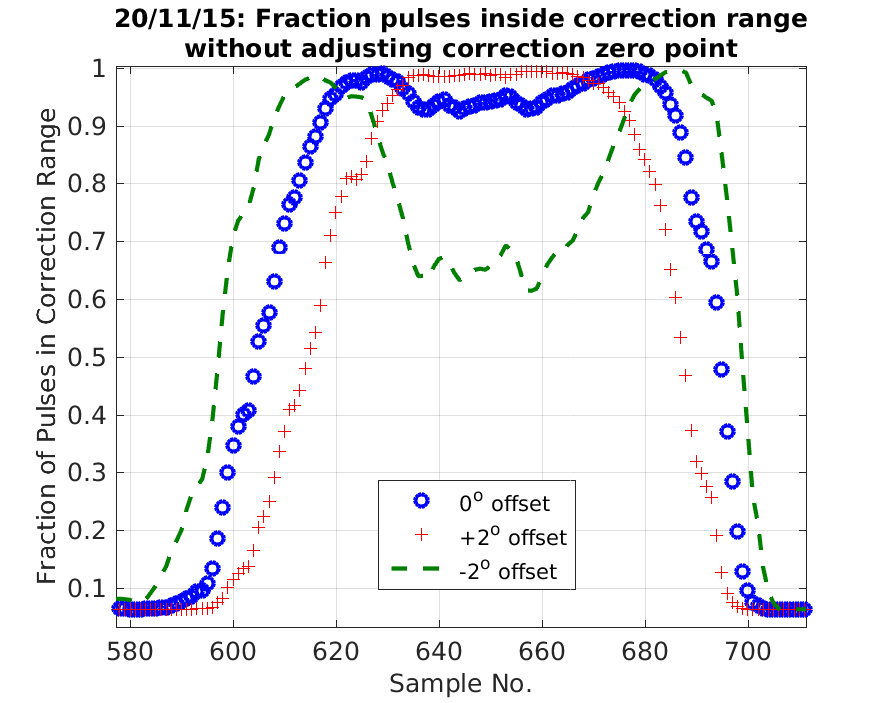
\includegraphics[width=0.75\textwidth]{Figures/feedforward/longFF_fractInRange}
  \caption{Fraction of pulses outside the correction range along the pulse. [TODO: Plot confusing as it stands due to sample range chosen]}
  \label{f:longFF_fractInRange}
\end{figure}

However, as to date this offset has been set up manually small deviations from the ideal case are possible. Figure \ref{f:longFF_fractInRange} also shows the fraction of pulses within the correction range if there is a static two degree offset in the upstream phase. In this case as many as 39\% of pulses are outside the correction range within the normally correctable central region of the pulse. To mitigate these effects and to get the largest reduction in jitter possible within each individual dataset the centring of the upstream phase in the correction range on the FONT5a board is normally adjusted between datasets. As a consequence of this differences in the upstream phase between datasets are not removed in the corrected downstream phase, as the zero point for the PFF correction is effectively moving with the phase drifts during the afternoon. These remaining slow drifts could be removed at CTF3 using a secondary ``slow phase feedback", also utilising the TL2 chicane, which is the focus of Section \ref{s:slowCorr}.

The accuracy to which the channel offset for the upstream phase has been selected can be inferred by comparing the mean downstream phase in each dataset with the correction on (red) and off (blue) in Figure \ref{f:longFF_noMeanSubHistory}. In the ideal case the mean phase should be identical with the PFF system on and off, so that the full correction range is being used to correct jitter about the mean as mentioned previously. Although this is the case for some datasets, such as the 15:38 dataset, a clear offset between the two is often present, most visible in the datasets between 16:39 and 16:50 in which the corrected phase is clearly shifted several degrees with respect to the uncorrected phase. The offset in each dataset is plotted in Figure \ref{f:longFF_phaseOffset} [TODO: Change to table?]. In the region between 16:39 and 16:50 the offset falls below \(-3^\circ\). The mean offset across the combined dataset is \(-1.4^\circ\) [TODO: Calc error, weight by datset lengths]. Even with the clearly non-optimal set point for the offset there should be almost no effect on the correction [TODO: calculate, plot]. Nevertheless, implementing an automatic procedure to set the offset optimally in the FONT5a DAQ would be a useful improvement to the PFF setup procedure and this will be pursued for future PFF attempts in 2016.

\begin{figure}
  \centering
  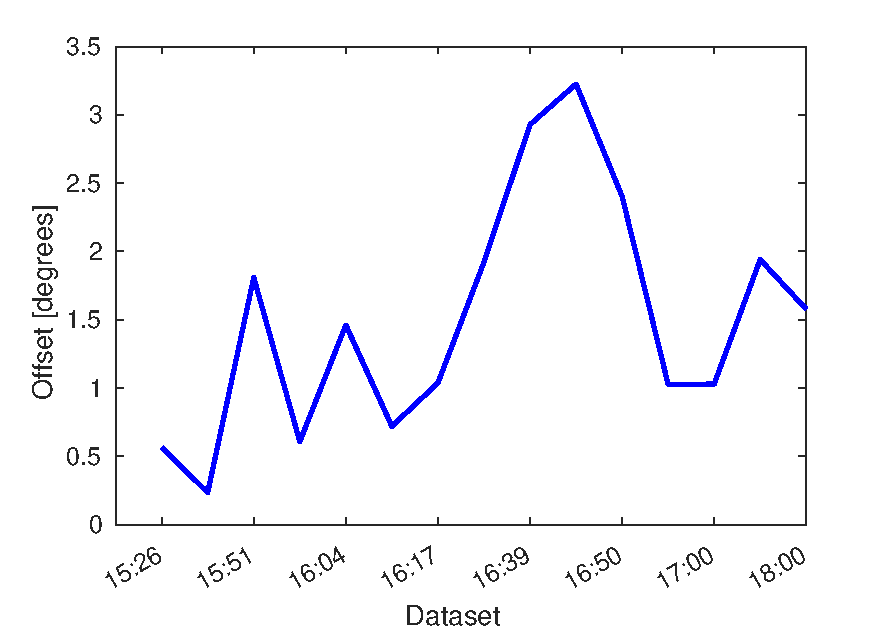
\includegraphics[width=0.75\textwidth]{Figures/feedforward/longFF_phaseOffset}
  \caption{Offset between downstream phase with FF off and FF on.}
  \label{f:longFF_phaseOffset}
\end{figure}


\subsection{Gain Stability}
\label{ss:longFF_gain}

Another PFF parameter that has been set up largely empirically to date is the correction gain. Historically, the gain set point for the PFF prototype has been determined by a combination of viewing the results of gain scans (Section \ref{s:gainScans}) and by observing the flatness of the corrected downstream phase in online displays of the phase monitor signals. If the applied gain is too large this can be quickly seen in the online monitors as the PFF system will act to invert the original phase sag along the pulse, for example. In this way it is relatively simple to find approximately the correct gain set point and further fine-tuning is done by varying the gain in small steps between datasets. In later PFF attempts this approach was complimented by implementing an online display of the optimal gain given the current measured upstream and downstream phase jitters and correlation (in the monitor presented in Section \ref{ss:sisSetup}), although this only gives a representative value when the PFF system is turned off. However, in this section it will be shown that due to instabilities in the beam conditions at CTF3 there are large variations in the optimal gain between datasets, and these variations are rarely accurately followed in the PFF setup when using this empirical approach. An automatic gain optimisation procedure is therefore another area of improvement for future PFF attempts. Particularly if the gain was automatically updated in real time during long datasets a significant reduction in jitter could be achieved, as will be seen in the remainder of this chapter.

The optimal gain depends on the downstream-upstream phase jitter ratio and the downstream-upstream phase correlation (Section \ref{ss:theoryGain}). In Figures \ref{f:longFF_noMeanSubHistory} and \ref{f:longFF_history} large differences in the phase stability in each dataset are clearly visible, comparing for example the large phase jumps in the 15:26 and 16:50 datasets to the comparatively calm periods at 15:38 and 16:17. This is summarised in Figure \ref{f:longFF_jitFFOff}, which shows the upstream and downstream (with PFF off) phase jitter across the 5--10 minute time period of each dataset. Over the course of the afternoon the mean upstream and downstream phase jitter both vary by around a factor two --- the upstream jitter between \(0.6\pm^\circ\) in the 16:17 dataset and \(1.1\pm^\circ\) at 16:22, and the downstream jitter between \(0.7\pm^\circ\) at 15:38 and \(2.2\pm^\circ\) at 16:50. [TODO: error] Given the same correlation, a factor two increase in the uncorrected downstream jitter also doubles the corrected downstream phase jitter that can be achieved with the PFF system.

Also of key importance for the PFF correction is that not only are there large variations in jitter between datasets but additionally in the downstream-upstream jitter ratio (dashed line in Figure \ref{f:longFF_jitFFOff}). In fact, the only dataset in which the upstream and downstream jitter is comparable is the record 15:38 dataset (with a ratio of 1.1). In all other datasets the downstream jitter is more than 1.3 times larger than the upstream jitter, reaching a maximum amplification of 2.2 in the 16:50 dataset. The mean ratio across the 15 datasets is 1.5 with a standard deviation of 0.3. [TODO: errors]

\begin{figure}
  \centering
  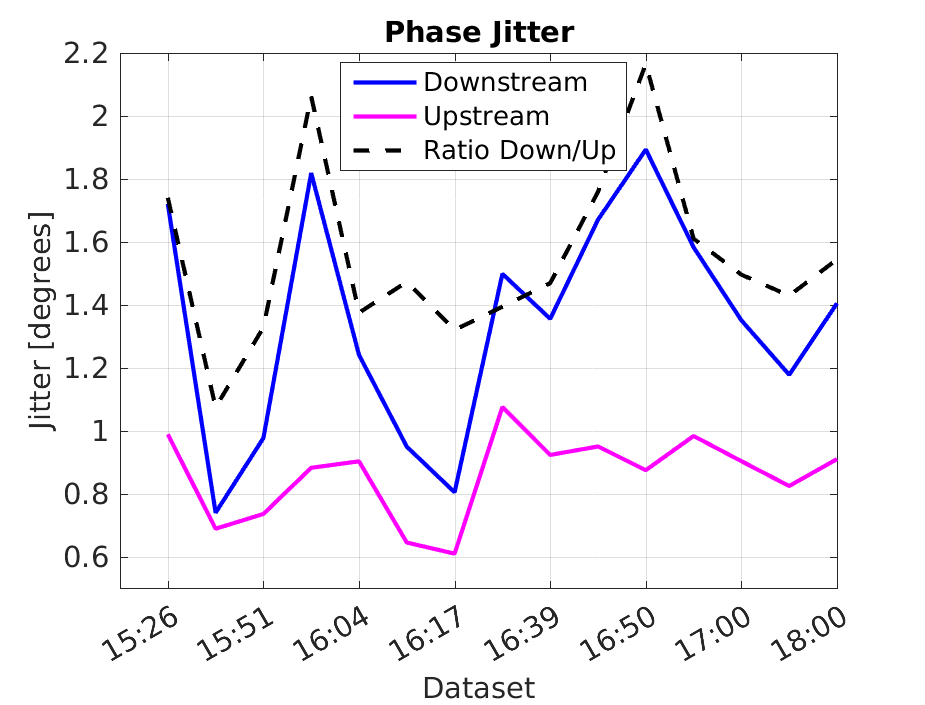
\includegraphics[width=0.75\textwidth]{Figures/feedforward/longFF_jitDatSetFFOff}
  \caption{Upstream and downstream phase jitter in each data set.}
  \label{f:longFF_jitFFOff}
\end{figure}

As well as the jitter ratio, the upstream-downstream phase correlation also varies between datasets, as shown in Figure \ref{f:longFF_corrFFOff}. The worst correlation is \(0.80\pm0.04\) in the 15:26 dataset and the best \(0.96\pm0.03\) in the 16:54 dataset. Although this has a much smaller 20\% effect on the optimal gain than the factor 2 variation in jitter ratio, it has a large effect on the theoretical jitter improvement that can be achieved with the PFF system due to the dependence on the correlation squared in Equation \ref{e:theoretJitOptGain}. With 80\% phase correlation only a theoretical factor 1.7 reduction in the downstream phase jitter can be achieved, whereas with 96\% correlation this is increased to a factor 3.6. 

\begin{figure}
  \centering
  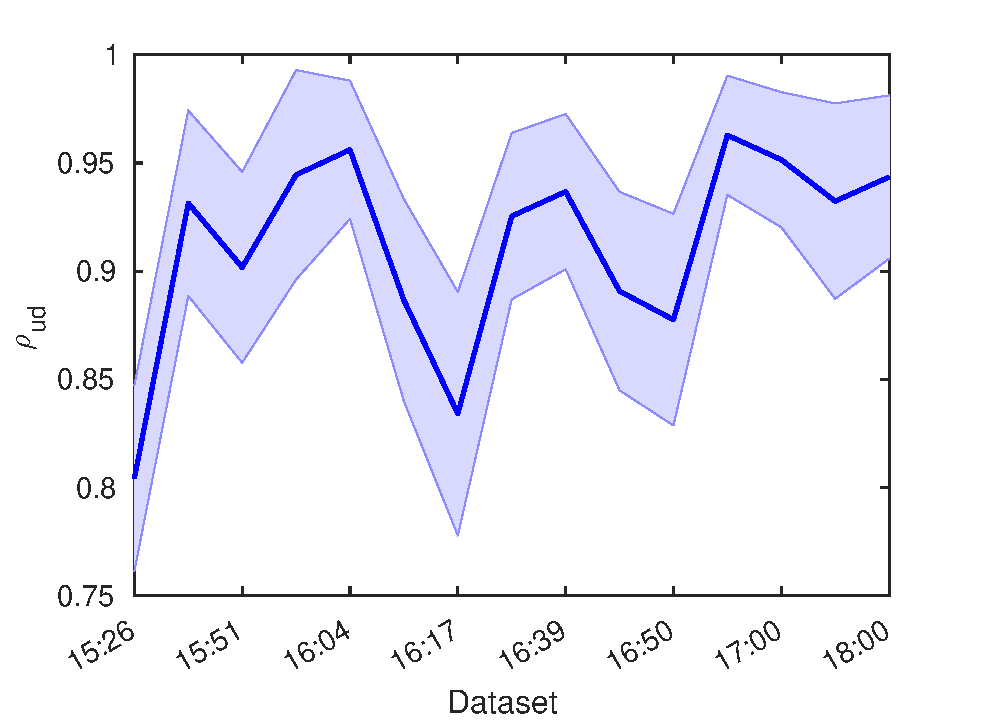
\includegraphics[width=0.75\textwidth]{Figures/feedforward/longFF_corrFFOff}
  \caption{Upstream-downstream mean phase correlation in each dataset with PFF off.}
  \label{f:longFF_corrFFOff}
\end{figure}

There is no observed dependence of the phase jitter ratio on the phase correlation, as shown in Figure \ref{f:longFF_corrVsJitRat}, so the effects of varying correlation and jitter ratio on the optimal gain are independent. [TODO:why?]. They combine to give the optimal gain plotted in Figure \ref{f:longFF_gain} (red line). As it is dominated by the differences in jitter ratio, the gain also varies by close to a factor two, varying from 1.00 in the 15:38 dataset to 1.95 in the 16:00 dataset. The real gain factor that was actually used in the dataset is also plotted, in blue. Although in places the empirically derived gain that was used follows the trend of the optimal gain, the changes are much smaller and it is clear that the real gain was systematically lower than the optimal gain. The smallest gain actually used was 1.06 (at 15:51) and the largest 1.34 (15:26 and 16:00), with an overall mean across the afternoon of 1.16 compared to the optimal value of 1.41. The impact this has on the achievable corrected downstream phase jitter is discussed in the next section.  

\begin{figure}
  \centering
  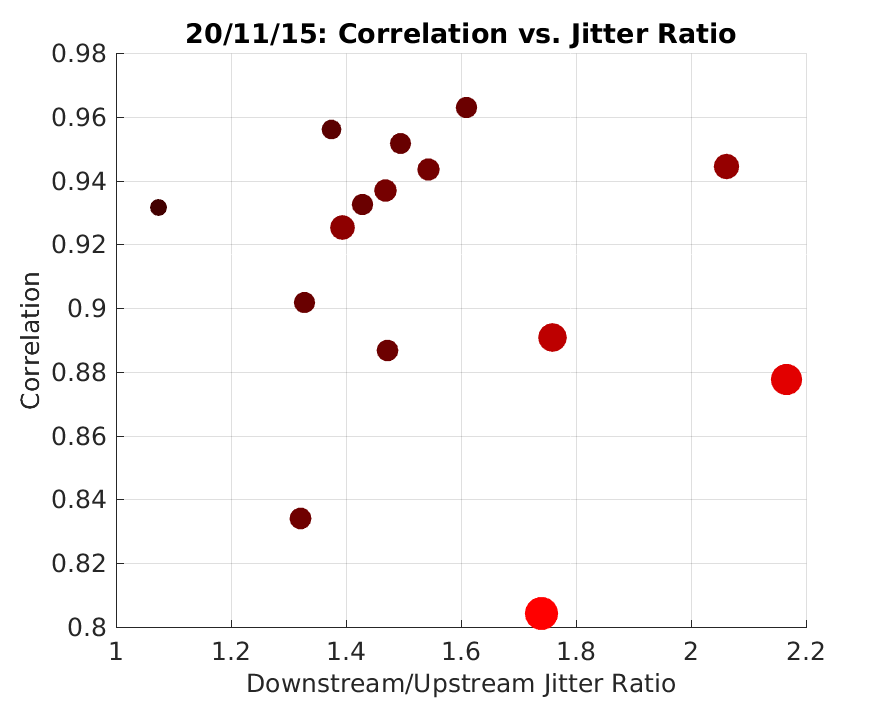
\includegraphics[width=0.75\textwidth]{Figures/feedforward/longFF_corrVsJitRat}
  \caption{Correlation vs. phase jitter ratio.}
  \label{f:longFF_corrVsJitRat}
\end{figure}

\begin{figure}
  \centering
  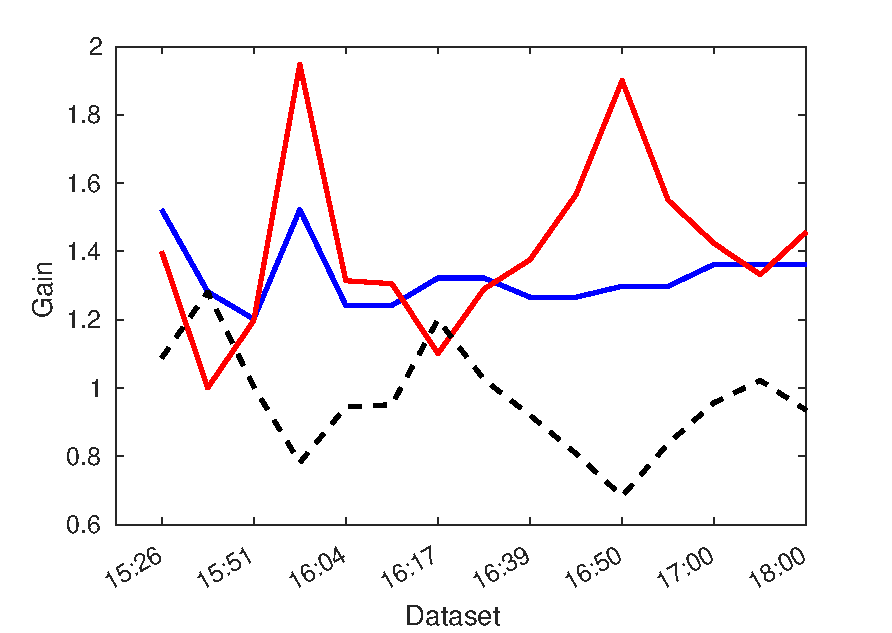
\includegraphics[width=0.75\textwidth]{Figures/feedforward/longFF_gain}
  \caption{Gain used in each dataset compared to the optimal gain.}
  \label{f:longFF_gain}
\end{figure}



\subsection{Individual Dataset Results}
\label{ss:longFF_singleResults}

It has been shown that the frequent drifts in both phase and downstream-upstream phase jitter ratio have not been optimally taken in to account in the PFF setup in terms of the used offset and gain. Nevertheless, even with a sub-optimal setup a large reduction in the downstream phase jitter can be achieved in all datasets. In the remainder of this chapter it will be shown that considering these constraints the PFF system is achieving close to peak performance, as well as highlighting the benefit that more accurate gain and offset control would have. Here the results in each individual dataset will be compared, before considering the combined dataset as a whole in the following section.

Firstly referring back to Figure \ref{f:longFF_corrVsJitRat}, the size (area) and colour of the markers in the plot depend on the corrected downstream jitter that could be achieved in that dataset using the optimal gain. Small, black markers correspond to the lowest theoretical jitter and large, red markers to the largest theoretical jitter. This is to emphasise again that it is a compromise between high correlation and low initial downstream jitter (and by extension low downstream-upstream jitter ratio) that gives the best conditions for the PFF correction (at least in terms of demonstrating \(0.2^\circ\) phase stability at CTF3, in principle high correlation is the only requirement for the secondary goal of achieving a factor 10 reduction in phase jitter). There are seven datasets with an achieved correlation of above the 93\% seen in the 15:38 record result, for example, but they yield worse theoretical corrections as 15:38 remains the only dataset in which a high correlation and low upstream-downstream jitter amplification have been achieved at the same time.

Figure \ref{f:longFF_datSetJitSim} then shows the theoretical limit on the corrected downstream jitter chronologically for each dataset, both with the optimal gain and the real used gain. Theoretically, the downstream phase jitter could be reduced by up to a further 0.2 degrees in the datasets with the largest difference between the optimal gain and real gain used (16:00 and 16:50). In most datasets the effect is much smaller than this, with an overall mean jitter degradation of \(0.07\pm0.02^\circ\) in each dataset expected compared to using the optimal gain. Only the 15:38 dataset has a theoretical (both with the optimal and actual gain) corrected downstream jitter of below \(0.3^\circ\) but in 10 out of 15 datasets below \(0.5^\circ\) jitter could have been achieved with optimal gain (or in 7 out of 15 with the real dataset gain). Further improvements not only in the peak phase propagation conditions achieved so far but also clearly on the stability of the phase propagation are therefore needed to demonstrate CLIC level phase stability both on short and long time scales at CTF3.

\begin{figure}
  \centering
  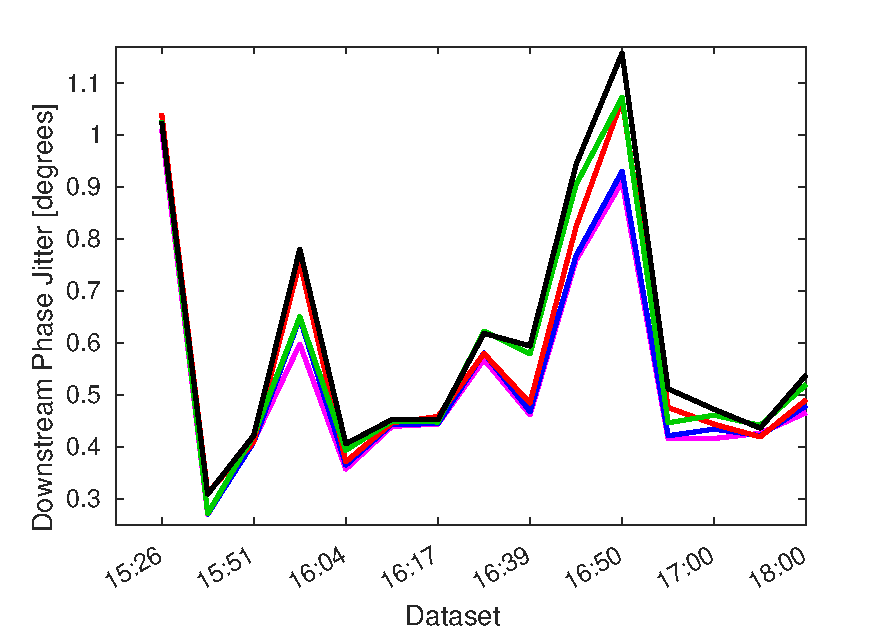
\includegraphics[width=0.75\textwidth]{Figures/feedforward/longFF_datSetJitSim}
  \caption{Theoretical corrected downstream jitter with optimal and used gain.}
  \label{f:longFF_datSetJitSim}
\end{figure}

Finally, the achieved downstream jitter with the real PFF system are presented in Figure \ref{f:longFF_jitDatSet}, along with the uncorrected downstream and upstream jitter and the simulated results with the actual gain used. In most datasets the real corrected downstream jitter is very close to the expected result from the simulation. However, there is a region 16:17 and 16:50 where the results are worse than expected. The largest difference is in the 16:44 dataset, where a jitter of \(1.11^\circ\) was achieved but \(0.88^\circ\) was expected in the simulation (or \(0.76^\circ\) if the gain was optimal). [TODO: Why? Possible explanation - 16:44 dataset has largest offset. Check simulation taking offset in to account]. Nevertheless, the downstream phase jitter is reduced in every dataset, with a maximum reduction factor of 3.2 in the 16:05 dataset (in which the highest correlation of 96\% was achieved). Attempts to demonstrate a larger reduction factor, closer to the CLIC specification of an order of magnitude, are presented in Section \ref{s:pffNovelSetups}.

\begin{figure}
  \centering
  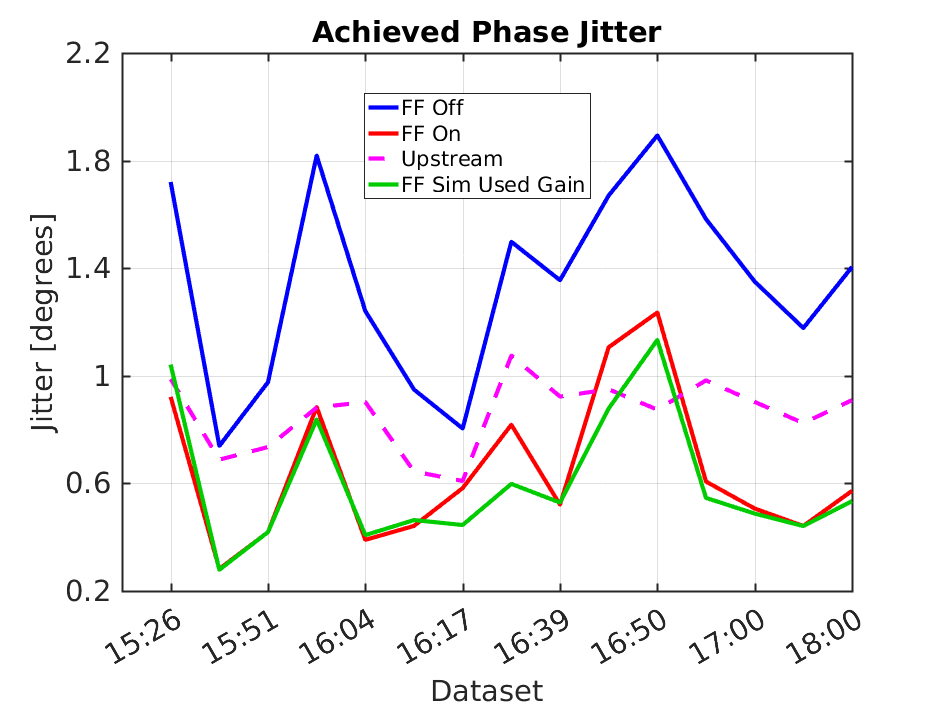
\includegraphics[width=0.75\textwidth]{Figures/feedforward/longFF_jitDatSet}
  \caption{Real corrected downstream jitter.}
  \label{f:longFF_jitDatSet}
\end{figure}


[TODO: Results along pulse?]
[TODO: Table of results]

\subsection{Combined Dataset Results}
\label{ss:longFF_combinedResults}

mean subtraction
jump in downstream phase

\begin{figure}
  \centering
  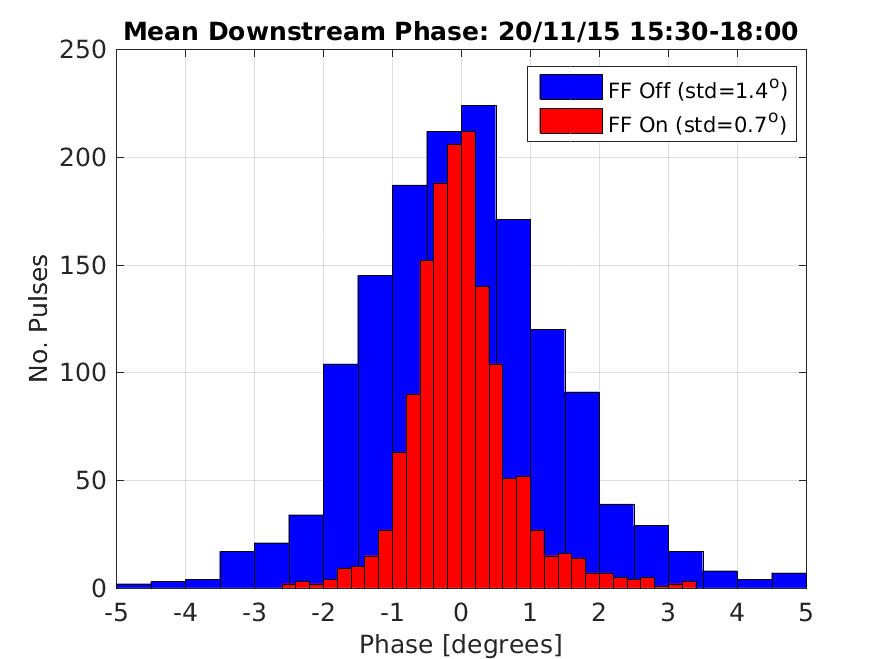
\includegraphics[width=0.75\textwidth]{Figures/feedforward/longFF_histDownstreamPhase}
  \caption{Histogram showing overall distribution of downstream phase with FF off and on.}
  \label{f:longFF_histDownstreamPhase}
\end{figure}

\begin{figure}
  \centering
  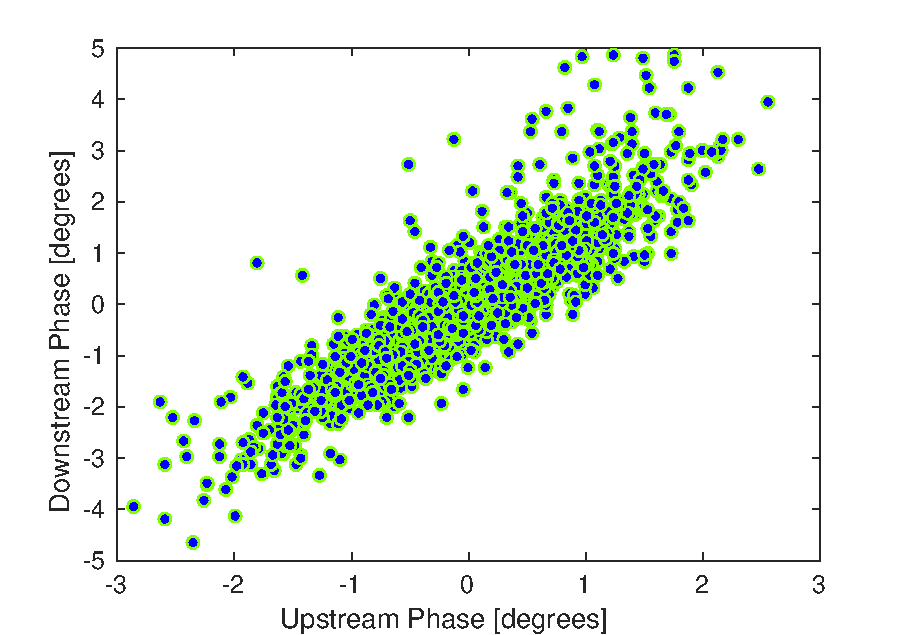
\includegraphics[width=0.75\textwidth]{Figures/feedforward/longFF_scatterFFOff}
  \caption{Downstream phase vs. upstream phase with FF off.}
  \label{f:longFF_scatterFFOff}
\end{figure}

\begin{figure}
  \centering
  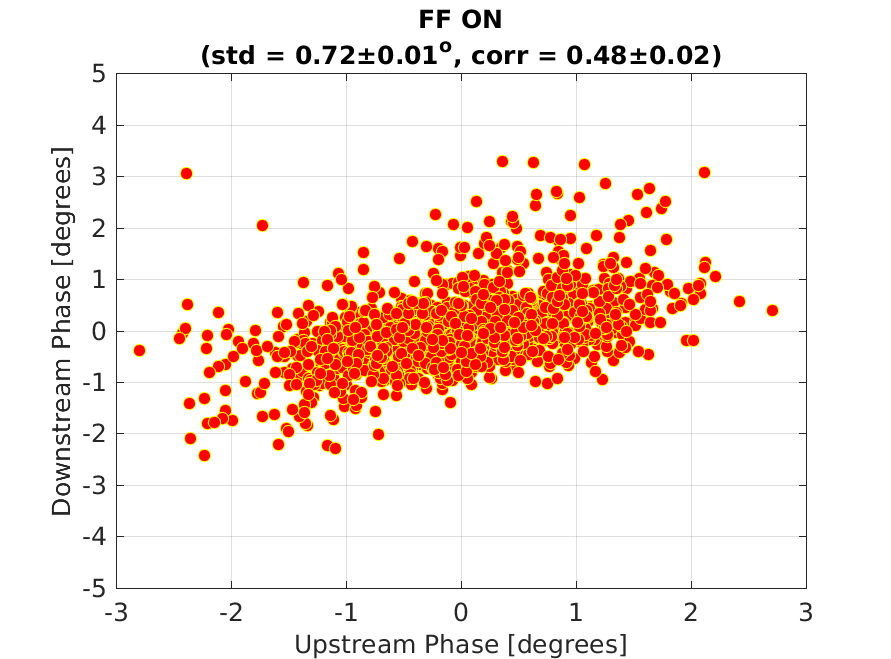
\includegraphics[width=0.75\textwidth]{Figures/feedforward/longFF_scatterFFOn}
  \caption{Downstream phase vs. upstream phase with FF on.}
  \label{f:longFF_scatterFFOn}
\end{figure}

\begin{figure}
  \centering
  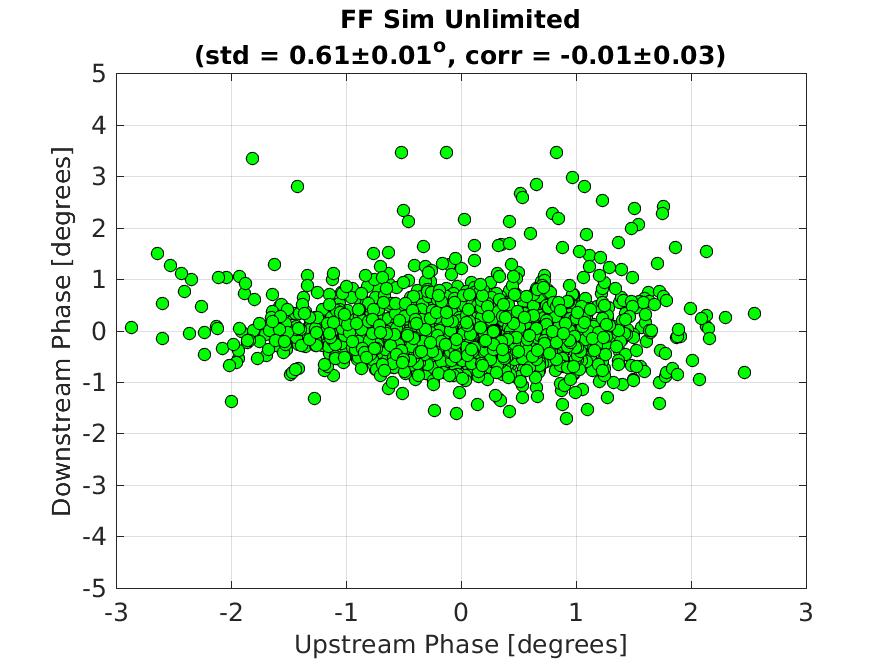
\includegraphics[width=0.75\textwidth]{Figures/feedforward/longFF_scatterFFSimOpt}
  \caption{Downstream phase vs. upstream phase with FF simulated at optimal gain.}
  \label{f:longFF_scatterFFSimOpt}
\end{figure}

\begin{figure}
  \centering
  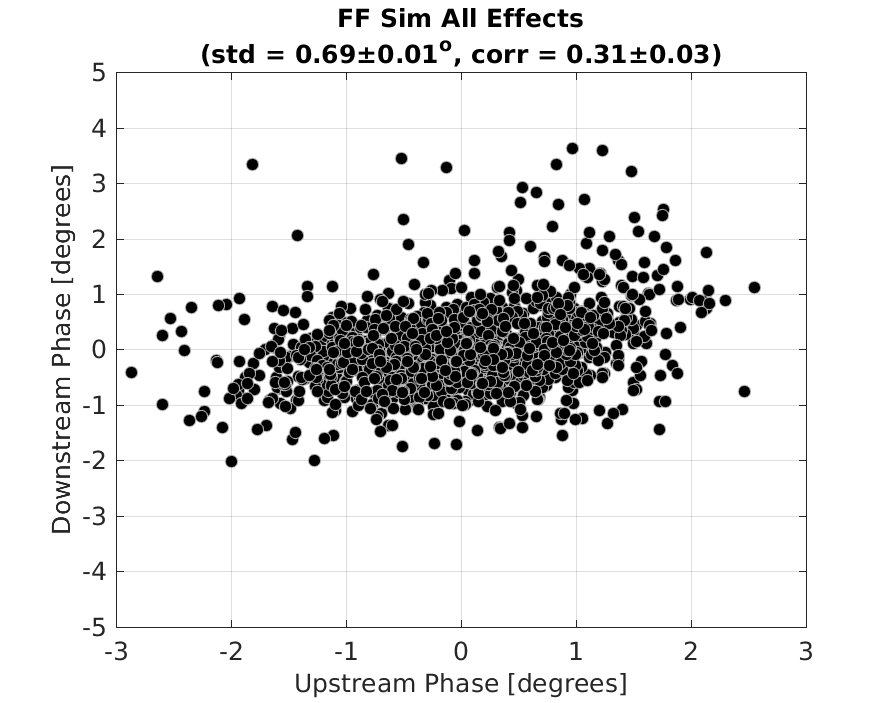
\includegraphics[width=0.75\textwidth]{Figures/feedforward/longFF_scatterFFSimReal}
  \caption{Downstream phase vs. upstream phase with FF simulated with actual gain used.}
  \label{f:longFF_scatterFFSimReal}
\end{figure}

\begin{table}
  \begin{center}
    \begin{tabular}{| c | c | c | c |}
	   \hline
       Correction Status & Upstream Jitter & Downstream Jitter & Correlation \\ \hline
       FF Off & \(0.88\pm0.02^\circ\) & \(1.40\pm0.03^\circ\) & \(0.89\pm0.01\) \\
	   FF On & \(0.86\pm0.02^\circ\) & \(0.72\pm0.01^\circ\) & \(0.48\pm0.02\) \\
	   FF Sim Opt Gain & \(0.88\pm0.02^\circ\) & \(0.61\pm0.01^\circ\) & \(-0.01\pm0.03\) \\
	   FF Sim Real Gain & \(0.88\pm0.02^\circ\) & \(0.68\pm0.01^\circ\) & \(0.35\pm0.02\) \\
	   FF Sim Offset & \(0.88\pm0.02^\circ\) & \(0.69\pm0.01^\circ\) & \(0.36\pm0.02\) \\
	   FF Sim 90\% Real Gain & \(0.88\pm0.02^\circ\) & \(0.72\pm0.01^\circ\) & \(0.46\pm0.02\) \\ \hline
    \end{tabular}
    \caption{Feedforward results using combined data from 20th November 2015.}
  	\label{t:LongFF}
  \end{center}
\end{table}



\newsection{pffNovelSetups}{Correction with Additional Jitter Source}

At CLIC the PFF system will be required to reduce the initial phase jitter by an order of magnitude, from 2 degrees to 0.2 degrees [REF]. With the initial phase jitter of typically 0.8 degrees at CTF3 it is not possible to demonstrate more than a factor 4 reduction in the jitter using the PFF prototype due to hardware limitations, more specifically due to the achieved phase monitor resolution of 0.14 degrees which limits the theoretical best possible correction to 0.2 degrees (Section \ref{s:resolution}). A secondary goal of the PFF prototype in addition to achieving the baseline goal of 0.2 degrees phase jitter is to demonstrate the factor 10 reduction in jitter relevant to CLIC. In order to do this additional sources of phase jitter must be added.

Clearly, the additional source must be prior to the upstream phase monitor in order to add an additional jitter component that is present in both the upstream and downstream monitors. The correlation between the resulting upstream and downstream phase must be  \(99.5\%\) in order for a factor 10 reduction in jitter to be possible (see Section \ref{ss:theoryJitter}). Two different methods to achieve this have been attempted --- firstly by varying the phases of all the klystrons in the injector and secondly by using the non-zero R56 stretching chicane (see Figure \ref{f:ctfLayout}) at the end of the CTF linac in order to intentionally add an energy component to the upstream phase (which propagates downstream).

\newsection{slowCorr}{Slow Correction}

As the PFF system has only a small range of \(\pm6^{o}\), a secondary ``slow phase feedback" or ``slow correction" has also been implemented at CTF3 to be able to remove larger drifts or static offsets in the downstream phase. In principle this slow correction can be used in conjunction with the PFF system to maximise its performance by keeping the mean uncorrected phase well-centred (zeroed) within its \(\pm6^{o}\) range so that the full power of the PFF amplifiers can be used to correct the fast pulse-to-pulse and intra-pulse phase jitter. If the beam phase were to drift away by \(15^{o}\), for example, the calculated PFF correction would saturate the amplifier across the full pulse length to give the maximal shift of \(6^{o}\). In this case the drift would be partially removed downstream but the PFF system would no longer have any effect on the phase jitter (as the output voltage to the kickers is constant in saturation rather than varying with the phase).

The design and results from the slow correction are discussed in this section. To date its main use has been to verify the ability to shift the beam phase in the TL2 chicane in early-2014 prior to the kicker amplifiers being available to commission the PFF system itself. The slow phase feedback has not yet been used in parallel with the PFF system apart from preliminary tests thus the results shown here are primarily a proof of principle. As PFF attempts have so far been predominantly taken in short datasets of up to a few hundred pulses any large drifts that arise can be manually removed between datasets, either by changing the correction setup (e.g. by changing the phase monitor phase shifters to re-zero the phase) or by re-establishing the previous beam conditions. The slow correction will however be an important tool for future attempts to demonstrate CLIC-level phase stability on time scales longer than a few minutes at CTF3.

\subsection{Implementation}
\label{ss:slowCorrMethod}

Ratio of corrector strengths for orbit closure.

\subsection{Results}
\label{ss:slowCorrResults}




